\documentclass[pra,onecolumn,floatfix,superscriptaddress,longbibliography,notitlepage, nofootinbib]{revtex4-1}
\usepackage[utf8]{inputenc}
\usepackage{amsmath}
\usepackage{amssymb}
\usepackage{tikz}
\usepackage{amsmath,amsfonts,amssymb}
\usetikzlibrary{3d}
\usetikzlibrary{arrows.meta}

\begin{document}

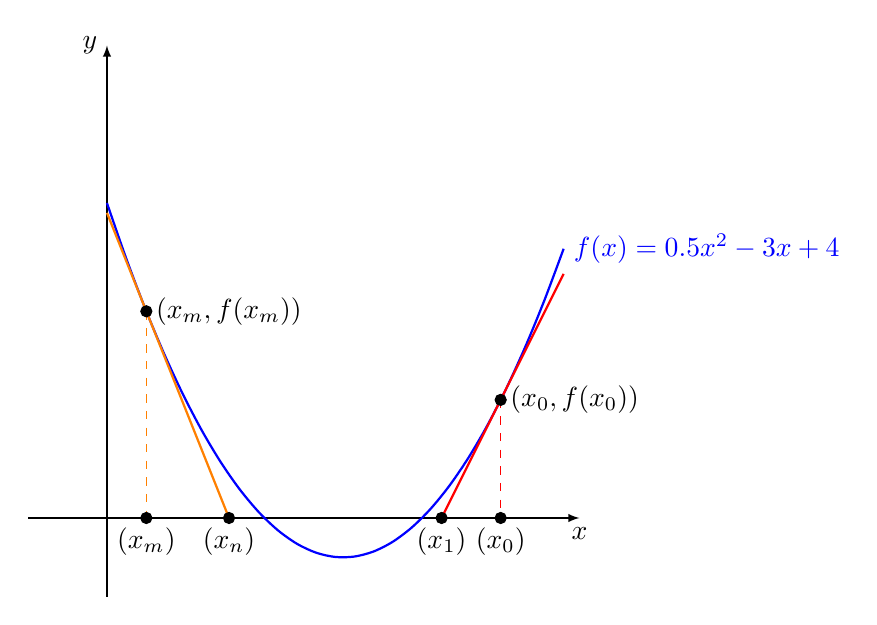
\begin{tikzpicture}[>=latex]
% Axes
\draw[->] (-1,0) -- (6,0) node[below] {$x$};
\draw[->] (0,-1) -- (0,6) node[left] {$y$};

% Function
\draw[blue, thick, domain=0:5.8, smooth, variable=\x] plot (\x, {0.5*\x^2 - 3*\x + 4}) node[right] {$f(x) = 0.5x^2-3x+4$};
\draw[red, thick, domain = 4.25:5.8, smooth, variable = \x] plot (\x, {2*\x - 8.5}) node[below right]{}; 
\draw[orange, thick, domain = 0:1.55, smooth, variable = \x] plot (\x, {-2.5*\x +3.875}) node[below]{}; 

% Tangent line
\draw[red, dashed] (5,1.5) -- (5,0) node[right] {};
\draw[orange, dashed] (0.5,2.625) -- (0.5,0) node[right] {};

% Initial guess
\filldraw[fill= black, draw=black] (5,1.5) circle (2pt) node[right] {$(x_0, f(x_0))$};
\filldraw[fill = black, draw=black] (5,0) circle (2pt) node[below] {$(x_0)$};
\filldraw[fill = black, draw = black] (4.25,0) circle (2pt) node[below] {$(x_1)$};
\filldraw[fill = black, draw = black] (0.5,2.625) circle (2pt) node[right] {$(x_m,f(x_m))$};
\filldraw[fill = black, draw = black] (1.55,0) circle (2pt) node[below] {$(x_n)$};
\filldraw[fill = black, draw =black] (0.5,0) circle (2pt) node[below] {$(x_m)$};
\end{tikzpicture}

\end{document}